\chapter{Vektorer og Matricer}
Dette appendix er skrevet med udgangspunkt i \citep{lial}

Lineær algebra kan blandt andet anvendes til at løse lineære ligningssystemer, hvilket især er i fokus dette projekt. De lineære ligningssystemer introduceres i Appendix \ref{afsnit:linlign}, og anvendes gennemgående i projektet.
En af de mest nyttige algoritmer til at løse sådanne ligningssystemer, er Gauss elimination, som også vil blive beskrevet i Appendix \ref{afsnit:linlign}. 
Dette Appendix vil gennemgå den grundlæggende teori for vektorer og matricer samt regneregler for dem, som lægger grundlaget for den senere teori i projektet.

\input{incl/main/lin_alg/matricer.tex}
%\subsection{Vectorer}
En bestemt type af matricer består kun af en søjle eller række, disse kaldes vektorer. 

\section{Regneoperationer med vektorer og matricer}

Da vektorer også er matricer vil regneregler for matricer også gælde for vektorer. I dette afsnit gennemgås først addition og skalering af matricer og senere gennemgås matrixmultiplikation.\\

\subsection{Addition og skalering}
Addition af matricer kan kun foretages for matricer med samme størrelse, da additionen laves ved at addere matrix-indgange på tilsvarende indgange.

\begin{defn}[Addition af matricer]
Lad $A, B, C$ være $m \times n$ matricer, så $C=A+B$. Da er den $i,j$'te indgang i $C$ givet ved $c_{i,j} = a_{i,j} + b_{i,j}$. 
\end{defn}


%Ved addition af to vektorer, placeres vektorerne i samme begyndelsespunkt, så de udspænder to sider af et parallelogram. Da følger af parallelogram-loven, at diagonalen af det fulde parallelogram er summen af de to vektorer.
%Repræsenteres  vektorene som en matrix, er summen af vektorene, en ny matrix, hvis $i$te indgang er summen af de to vektores $i$te indgange. 
%Bemærk derfor, at det ikke er muligt at lægge to vektorer sammen af forskellig dimension. Det er heller ikke muligt at finde summen af en søjle- og rækkevektor, selvom de har samme dimension.

%Addition af to vektorer kan repræsenteres grafisk med pile, ved at tage to ikke-nul vektorer $\vec{u}$ og $\vec{v}$ og forme et parallelogram med vektorene som parallelogrammets sider. I følge parallelogram loven vil diagonalen af parallelogrammet være de to vektor lagt sammen $\vec{u}+\vec{v}$.
%Mangler firgur 1.3 fra lial bogen

Tilsvarende kan vektorer også adderes som defineret i Definition \ref{def:add_vek}. Regning med vektorer kan yderligere repræsenteres geometrisk, hvor vektorer anses som pile med en retning i så mange dimentioner som der er indgange i vektoren.

\begin{defn}[Addition af to vektor]
Lad $\vec{v}, \vec{u}, \vec{w} \in \mathds{R}^n$, så $\vec{w}=\vec{u}+\vec{v}$, da er den $i$'te indgang i $\vec{w}$ givet ved $w_i = u_i + v_i$ for $i=1, \dots ,n$. 
%Lad $\underset{m \times 1}{A}$ og $\underset{m \times 1}{B}$ være to vektorer med samme størrelse. Da vil additionen af de to vektorer give en vektor, $\underset{m \times 1}{C}$, hvor hver komponent er summen af de tilsvarende komponenter i $\underset{m \times 1}{A}$ og $\underset{m \times 1}{B}$.
%\begin{align*}
%\underset{m \times 1}{A} = 
%\begin{bmatrix}
%a_{1,1}\\
%a_{2,1}\\
%\vdots \\
%a_{m-1,1}\\
%a_{m,1} \\
%\end{bmatrix}
%\qquad
%\underset{m \times 1}{B} = 
%\begin{bmatrix}
%b_{1,1}\\
%b_{2,1}\\
%\vdots \\
%b_{m-1,1}\\
%b_{m,1} \\
%\end{bmatrix}
%\end{align*} 
%\begin{align*}
%C=A+B=
%\begin{bmatrix}
%a_{1,1}\\
%a_{2,1}\\
%\vdots \\
%a_{m-1,1}\\
%a_{m,1} \\
%\end{bmatrix}
%+
%\begin{bmatrix}
%b_{1,1}\\
%b_{2,1}\\
%\vdots \\
%b_{m-1,1}\\
%b_{m,1} \\
%\end{bmatrix}
%=
%\begin{bmatrix}
%a_{1,1}+b_{1,1}\\
%a_{2,1}+b_{2,1}\\
%\vdots \\
%a_{m-1,1}+b_{m-1,1}\\
%a_{m,1}+b_{m,1} \\
%\end{bmatrix}
%\end{align*}
\label{def:add_vek}
\end{defn}
\begin{eks}
Betragt de to $4$ dimensionelle vektorer
\begin{align*}
\vec{v}=
\begin{bmatrix}
4\\
1\\
0\\
-5\\
\end{bmatrix}
%\hspace{3cm}
\vec{u}=
\begin{bmatrix}
7\\
4\\
-2\\
-5\\
\end{bmatrix}
\end{align*}
Deres sum er
\begin{align*}
\vec{v}+\vec{u}=
\begin{bmatrix}
4\\
1\\
0\\
-5\\
\end{bmatrix}
+
\begin{bmatrix}
7\\
4\\
-2\\
-4\\
\end{bmatrix}
=
\begin{bmatrix}
4+7\\
1+4\\
0-2\\
-5-4\\
\end{bmatrix}
=
\begin{bmatrix}
11\\
5\\
-2\\
-9\\
\end{bmatrix}
\end{align*}
\end{eks}

Skalarmultiplikation er en skalering af alle indgangene i en matrix med en bestemt skalar.


\begin{defn}[Matrixskalar]
Lad $A$ være en $m \times n$ matrix og $k$ en skalar. Da vil matricen $B$ defineret ved $B=k \cdot A$, være en $m \times n$ matrix med indgange $b_{i,j}=k\cdot a_{i,j}$. Skalaren $k$ kaldes en \textbf{matrixskalar}. Er $A$ en vektor kaldes $k$ en \textbf{vektorskalar}.
\end{defn}

%\begin{defn}[Vektor skalar]
%Lad $\vec{v}, \vec{u}$ være en vektorer i $\mathds{R}^n$, og $k$ en skalar, så $\vec{u} = k \cdot \vec{v}$, da er den $i$te indgang i $\vec{u}$ givet ved $u_i = k\cdot v_i$.
%\end{defn}

%Hvis en vektor kan lægges til en anden vektor, må det også være muligt at skalere den. Det vil sige multiplicere den med en konstant, eftersom $2\vec{v}=\vec{v}+\vec{v}$.\\ %giver god mening, men det lyder som et bevis
\begin{figure}[h]
\begin{center}
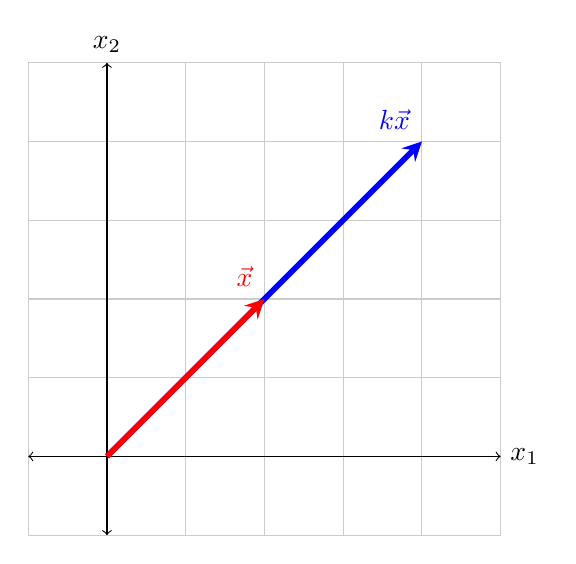
\begin{tikzpicture}
  \draw[thin,gray!40] (-1,-1) grid (5,5); %laver Grid
  \draw[<->] (-1,0)--(5,0) node[right]{$x_1$}; %x-aksen
  \draw[<->] (0,-1)--(0,5) node[above]{$x_2$}; %y-aksen
  \draw[line width=2pt,blue,-stealth](0,0)--(4,4) node[above left]{$k\vec{x}$}; %blå vektor
  \draw[line width=2pt,red,-stealth](0,0)--(2,2) node[above left]{$\vec{x}$}; %rød vektor
\end{tikzpicture}
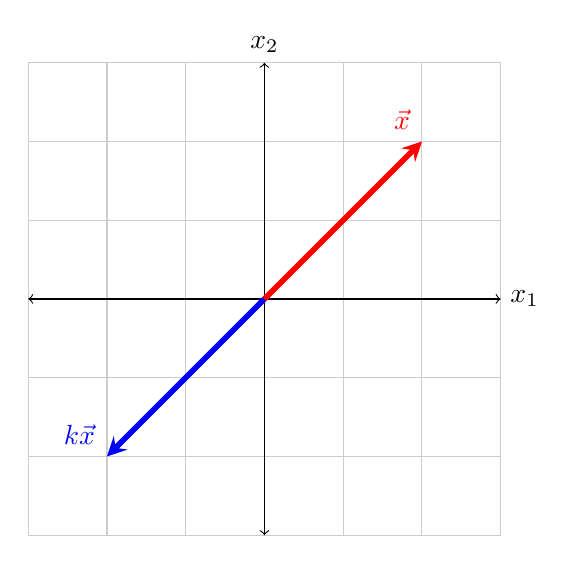
\begin{tikzpicture}
  \draw[thin,gray!40] (-3,-3) grid (3,3);
  \draw[<->] (-3,0)--(3,0) node[right]{$x_1$};
  \draw[<->] (0,-3)--(0,3) node[above]{$x_2$};
  \draw[line width=2pt,blue,-stealth](0,0)--(-2,-2) node[above left]{$k\vec{x}$};
  \draw[line width=2pt,red,-stealth](0,0)--(2,2) node[above left]{$\vec{x}$};
\end{tikzpicture}
\caption{Billede 1, viser skalar multiplikationen $k \cdot \vec{x}$, for $k=2$, mens $k=-1$ på billede 2.}
\end{center}
\label{fig:vektorskalar}
\end{figure}
%Derfor må den nye vektors komponenter være den originale vektors komponenter multipliceret med skalaren.


% da er et \textbf{vektor skalar} produktet af den vektorens komponenter multipliceret med konstanten.
%da er et \textbf{vektor skalar } givet ved,
%En \textbf{Vektor skalar} er produktet af en vektor $\vec{x}$
%som bliver multipliceret med en konstant $k$ kaldet skalar. Denne vektor peger i samme retning, men har en anden længde.
%\begin{align*}
%\vec{x}=\begin{bmatrix}
%%x_1\\
%%x_2\\
%%\vdots\\
%%x_{n-1}\\
%%x_n
%%\end{bmatrix}\\
%k\vec{x}=k\begin{bmatrix}
%x_1\\
%x_2\\
%\vdots\\
%x_{n-1}\\
%\end{bmatrix}=
%\begin{bmatrix}
%kx_1\\
%kx_2\\
%\vdots\\
%kx_{n-1}\\
%kx_n\\
%\end{bmatrix}
%\end{align*}

\begin{eks}
En vektor $\vec{x}$ med komponenterne $2$ og $3$ skal skaleres med skalaren $k=3$, hvilket gøres ved at multiplicere konstanten på begge komponenter.
\begin{align*}
\vec{x}=\begin{bmatrix}
2\\
3
\end{bmatrix}\qquad k=3\\
k\vec{x}=3
\begin{bmatrix}
2\\
3
\end{bmatrix}
=
\begin{bmatrix}
3\cdot2\\
3\cdot3
\end{bmatrix}
=
\begin{bmatrix}
6\\
9
\end{bmatrix}
\end{align*}
\end{eks}
%Da det at trække en vektor $\vec{v}$ fra, kan forstås som at lægge vektoren $(-1) \vec{v}$ til, kan vektor substation defineres ud fra addition og skalar multiplikation, se Figur \ref{fig:vektorskalar}.
%\begin{defn}[Vektor substation]
%Lad $\vec{u}, \vec{v} \in \mathds{R}^n$ være vektorer, %da er $\vec{u}-\vec{v}= \vec{u} + (-1) \vec{v}$.
%\end{defn}

%----------------------------------------------------

Givet to $m \times n$ matricer, $A$ og $B$, kan der udføres forskellige regneoperationer. \\

\begin{stn}
Lad $A$, $B$ og $C$ være $m \times n$ matricer, og lad $s$ og $t$ være tilfældige skalarer. Lad matricen $O$ være en nulmatrix.
Så gælder følgende
\begin{enumerate}[label=(\alph*)]
\item $A + B = B + A$
\item $(A + B) + C = A + (B + C)$
\item $A + O = A$
\item $A + (-A) = O$
\item $(st) A = s (tA)$
\item $s(A + B) = sA + sB$
\item $(s+t)A = sA + tA$
\end{enumerate}
\label{stn_regn}
\end{stn}

\begin{proof} 
(a) Det vises, at enhver indgang i $A + B$ er tilsvarende indgangen i $B + A$. Betragt indgangene $a_{i,j}$ og $b_{i,j}$. Summen af $a_{i,j} + b_{i,j}$ er det samme som $b_{i,j} + a_{i,j}$, jf. den kommutative lov. \\
(b) Det vises, at enhver indgang i $(A + B) + C$ er den samme som den tilsvarende indgang i $A + (B + C)$. Ligesom i (a) tages der udgangspunkt i indgang $(i,j)$. Summen af $(a_{i,j} + b_{i,j}) + c_{i,j}$ er det samme som $a_{i,j} + (b_{i,j} + c_{i,j})$. Ifølge den associative lov, er det uden betydning hvor paranteserne er placeret i et additionsudtryk. Derfor må indgangen $(i,j)$ i $(A + B) + C$ være lig indgang $(i,j)$ i $A + (B + C)$. \\
(c) For enhver indgang i $A$, $a_{i,j}$ skal denne adderes med $0$. $a_{i,j}+0=a_{i,j}$. Derfor må $A + O = A$. \\
(d) For enhver indgang i $A$, $a_{i,j}$ skal denne fratrækkes samme indgang i $A$, $a_{i,j}$. Da \\ $a_{i,j} - a_{i,j} = 0$, må $A + (-A) = O$. \\
(e) Her tages der udgangspunkt i (i,j)-indgangen i A, $a_{i,j}$. Det ses så, at udsagnet bliver til $(st)a_{i,j} = s(ta_{i,j})$ når flere tal multipliceres, er det lige meget i hvilken rækkefølge, jf. den associative lov. \\
(f) Hver indgang i A, $a_{i,j}$ lægges sammen med den tilsvarende indgang i B, $b_{i,j}$, dette giver venstresiden $s(a_{i,j}+b_{i,j})$. Da det er tilladt at multiplicere ind i en parantes, kan udtrykket også skrives $s(a_{i,j}+b_{i,j})=sa_{i,j}+sb_{i,j}$, i følge den distributive lov. \\
(g) På samme måde som før tages der udgangspunkt i (i,j)-indgangen i A, $a_{i,j}$. Udtrykket på venstresiden er så $(s+t)a_{i,j}$. Ligesom før, givet den distributive lov, kan der multipliceres ind i parantesen og dermed fås følgende, $(s+t)a_{i,j}=sa_{i,j}+ta_{i,j}$.
\end{proof}

\begin{eks}[Addition og skalering af matricer]
For at vise eksempler på nogle af ovenstående regneoperationer, tages der udgangspunkt i matricerne $A$ og $B$, samt skalaren $s$. Først ses addition af matricer og derefter skalering for at finde $s(A+B)$
\begin{align*}
A= \begin{bmatrix}
	2 & 3 & 4 \\
	5 & -2 & 1 	
\end{bmatrix}, \quad
B= \begin{bmatrix}
	1 & 2 & -1 \\
	-3 & 4 & 0
\end{bmatrix}, \quad
s=5
\end{align*}
Først udføres addition af matricer,
\begin{align*}
A+B= \begin{bmatrix}
	2 & 3 & 4 \\
	5 & -2 & 1 	
\end{bmatrix}  
+ \begin{bmatrix}
	1 & 2 & -1 \\
	-3 & 4 & 0
\end{bmatrix}
= \begin{bmatrix}
	3 & 5 & 3 \\
	2 & 2 & 1
\end{bmatrix}.
\end{align*}
Herfter udføres skalering af matricer,
\begin{align*}
s(A+B)= 5 \cdot \begin{bmatrix}
	3 & 5 & 3 \\
	2 & 2 & 1
\end{bmatrix}
= \begin{bmatrix}
	15 & 25 & 15 \\
	10 & 10 & 5
\end{bmatrix}.\\
\end{align*}
\end{eks}

%------------------------------------------
\subsection{Matrixmultiplikation}

%To vektorer af samme dimension kan prikkes sammen ved at multiplicere deres $i$te indgange med hinanden og så finde summen af produktorne
%\begin{defn}[Prikproduktet]
%Lad $\vec{v}, \vec{u} \in \mathds{R}^n$ være to vektorer, da er \textbf{prikproduktet} givet ved $\langle\vec{v},\vec{u}\rangle = \sum_{i=1}^n v_i \cdot u_i.$
%\end{defn}
%Et matrix-vektor produkt, er produktet af en $m\times n$ matrix og en $n$ dimensional vektor, og svare til en $m$ dimentional vektor , hvis $i$te indgang er prikproduktet af den $i$te række og den $n$ dimensionalle vektor. 
%Dette lægger grundlaget for hvordan matricer ganges sammen, eftersom en vektor også kan ses som en $n\times1$ matrix. 
Et matrix-vektor produkt, er produktet af en $m\times n$ matrix og en $n$ dimensional vektor, og svarer til summen af vektorskalar-produktet mellem den $j$te søjle i matricen, og den $j$te indgang i vektoren, for enhver søjle i matricen.
\begin{defn}[Matrix-vektor produkt]
Lad $A$ være en $m\times n$ matrix og $\vec{v}\in \mathds{R}^n$. 
Da vil $A \vec{v} = \sum_{j=1}^n \vec{A_j}v_j = \vec{u}$, hvor $\vec{u} \in \mathds{R}^m$.
%Lad $A$ være en $m\tiems n$ matrix og $\vec{v}\in \mathds{R}^n$ vektor. Så skrives \textbf{Matrix-vektor produktet} $A\vec{x}$, som produktet af søjlerne $\vec{A_j}$ i $A$ og de tilsvarende komponenter i $\vec{x}$. Dette kræver at matricen har samme antal søjler som vektoren har komponenter, hvilket er defineret med $n$.
%\begin{align*}
%A\vec{x}&=x_1\vec{A}_1+x_2\vec{A}_2+ \dots +x_{n-1}\vec{A}_{n-1}+x_n\vec{A}_n \\
%&=
%\begin{bmatrix}
%x_1a_{1 1}+x_2a_{1 2}+\dots +x_{n-1}a_{1 n-1}+x_na_{1 n} \\
%x_1a_{2 1}+x_2a_{2 2}+\dots +x_{n-1}a_{2 n-1}+x_na_{2 n}\\
%\vdots\\
%x_1a_{m-1 1}+x_2a_{m-1 2}+\dots +x_{n-1}a_{m-1 n-1}+x_na_{m-1 n} \\
%x_1a_{m 1}+x_2a_{m 2}+\dots +x_{n-1}a_{m n-1}+x_na_{m n}
%\end{bmatrix}
%=
%\begin{bmatrix}
%\vec{a}_1\vec{x}\\
%\vec{a}_2\vec{x}\\
%\vdots\\
%\vec{a}_{m-1}\vec{x}\\
%\vec{a}_m\vec{x}
%\end{bmatrix}.
%\end{align*}
\label{def:matrixvektorprodukt}
\end{defn}
Bemærk at en $m \times n$ matrix kun kan multipliceres med en $n$ dimensionel søjlevektor ud fra Definition \ref{def:matrixvektorprodukt}. Produktet mellem en $m$ dimensionel rækkevektor og en $m \times n$ matrix, kan defineres på samme måde, så resultatet bliver en $n$ dimensionel vektor. 
Et særtilfælde af en matrix-vektor mulitiplikation er, når to vektorer multipliceres sammen. Dette kaldes et prikprodukt.
\begin{defn}[Prikproduktet]
Lad $\vec{v}, \vec{u} \in \mathds{R}^n$ være to vektorer, da er \textbf{prikproduktet} givet ved $\langle\vec{v},\vec{u}\rangle = \sum_{i=1}^n v_i \cdot u_i = \vec{v}^T \cdot \vec{u} $
\end{defn}
\begin{eks}
Betragt en $2 \times 3$ matrix og en $2$ dimentionel søjlevektor
\begin{align*}
A=
\begin{bmatrix}
1 & 4\\
2 & 5\\
3 & 6
\end{bmatrix}
\qquad
\vec{x}=
\begin{bmatrix}
7\\
8
\end{bmatrix}
\end{align*}
Da vil deres produkt være
\begin{align*}
A\vec{x}= \begin{bmatrix}
1 & 4\\
2 & 5\\
3 & 6
\end{bmatrix}
\begin{bmatrix}
7\\
8
\end{bmatrix}
=
7
\begin{bmatrix}
1\\
2\\
3
\end{bmatrix}
+ 8
\begin{bmatrix}
4\\
5\\
6
\end{bmatrix}=
\begin{bmatrix}
7\\
14\\
21
\end{bmatrix}
+
\begin{bmatrix}
32\\
40\\
48
\end{bmatrix}
=
\begin{bmatrix}
39\\
54\\
69
\end{bmatrix}
\end{align*}
\end{eks}
Et produkt af to matricer defineres herunder. 
\begin{defn} [Matrix produkt]
Lad $A$ være en $m \times n$ matrix og $B$ være en $n \times p$ matrix. Da er produktet $A \cdot B$ en $m \times p$ matrix, hvor indgangene er givet ved: 

$$(AB)_{i,j} = \vec{a}_i \cdot \vec{B}_j$$

hvor $\vec{a}_i$ er den $i$'te række i $A$, og $\vec{B}_j$ er den $j$'te søjle i $B$
\label{def:(matrixprodukt)}
\end{defn}
Det er vigtigt, at antallet af søjler i $A$ er det samme som antallet af rækker i $B$. Er dette ikke tilfældet, så er matrix produktet ikke defineret. Matrix produktet er oftest ikke kommutativt. Ligningen $AB=BA$ er derfor ikke altid gældende. 
\begin{eks}
Der tages udgangspunkt i to matricer $A$ og $B$. 
\begin{align*}
\underset{2 \times 3}{A}= \begin{bmatrix}
	\bf{1} & \bf{3} & \bf{-2} \\
	5 & 4 & 0 	
\end{bmatrix},
\underset{3 \times 4}{B}= \begin{bmatrix}
	\bf{2} & 3 & -1 & 3 \\
	\bf{1} & 4 & 5 & 5\\
	\bf{1} & 0 & 4 & 2
\end{bmatrix}  
\end{align*}
For at beregne indgang $(1,1)$ benyttes række $1$ i $A$ og søjle $1$ i $B$. 
$$ab_{1,1}=1\cdot 2+3\cdot 1-2 \cdot 1 = 3$$ 
De resterende indgange beregnes på samme måde. 
Matrix produktet af $A$ og $B$ er altså givet ved:
\begin{align*}
\underset{2 \times 4}{AB}= \begin{bmatrix}
	\bf{3} & 15 & 6 & 14 \\
	14 & 31 & 15 & 35
\end{bmatrix}  
\end{align*}
\end{eks}
